
\chapter{Introduction}
\label{sec:Introduction}
%Thesis high level overview (structure - goals - audience ...)

This chapter will start by giving insight into the problem and motivation behind this
thesis; it continues with an outlining of the contributions this research project provides. Lastly, the structure of the document is described.


\section{Problem and motivation}


Information has become the most valuable resource in modern society. From children to seniors, from New Zealand to Canada, a very large portion of the current human population have shared in some extend part of their life by technological means. This is a fact, no doubts. That fact opens unquantifiable possibilities for science. Especially Computer Science with topics such as Information Retrieval (IR), Machine Learning (ML), Natural Language Processing (NLP), Semantic Web, and the list goes on. The era of data analysis is just starting. 


Having a notion of people’s thoughts has always been an essential asset for the decision-making processes in many business models. Even before the existence of the World Wide Web, people used to ask questions about products recommendations or opinions about events such as local elections. But with the beginning of the Internet Era, societies started to use the common wealth of knowledge found on forums, blogs, and social media network services as an important source of opinions~\cite{pang2008opinion}. These opinions may come from customers simply sharing their experience with a product or from well-known professionals writing elaborated reviews. The Internet became a valuable pool of experiences available for everyone to use.

\clearpage

\begin{figure}
    \centering
    \caption[Social network user growth projections]{Social network user growth projection 2010 - 2018{~\cite{stat2018}}}
    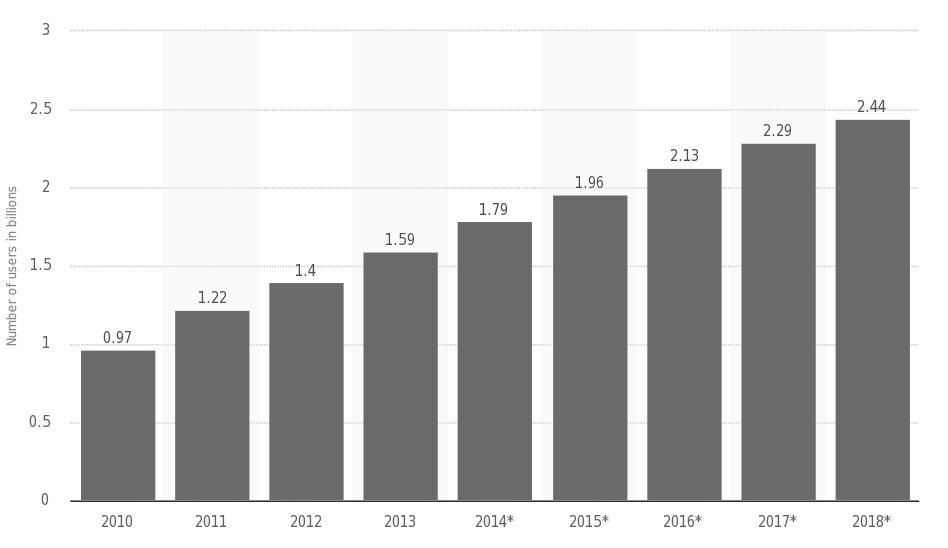
\includegraphics[width=\linewidth]{01_social_net_growth}
    \label{fig1:social_net_growth}
\end{figure}

In \autoref{fig1:social_net_growth} the number of social network users worldwide from 2010 to 2014 with projections until 2018 is represented. By 2018 the projection shows an astonishing amount of 2.44 billion users on social media networks, this is more than 30\% of the world's population. However, data generated from systems must be mined and analyzed to represent valuable information for interested parties. This master thesis aims to explore an approach called "Entity Based Sentiment Classification" to tackle this challenge.  

As shown on \autoref{fig1:social_net_growth} in the past few years, there has been an increase in the usage of social networking services such as Twitter. Twitter, as a micro-blogging system, allows users
to publish tweets of up to 140 characters in length to tell others what they are doing, what they are
thinking, or what is happening around them. Therefore, companies and media organizations are constantly looking for ways of extracting public opinions and feelings about their products and services~\cite{kouloumpis2011twitter}. The nature of the tweets (short and usually meaningful in the context of marketing) allows researchers to exploit different data mining and sentiment analysis approaches. Projects like Twitratr\footnote{\url{http:www.twitrratr.com}}, streamcrab \footnote{\url{http:www.streamcrab.com}}, and Talend\footnote{\url{http:www.talend.com}} are examples of services intending to obtain sentiment information from tweets.

\clearpage

\autoref{tab:tweets_sentiment} shows two example tweets together with their corresponding
sentiment. The first tweet expresses a positive sentiment, containing one positive noun \textit{happy} and one positive emoji :D. The sencond tweet indicates negative sentiment based on the hashtag \textit{\#sad } and emoji :(.

\begin{table}[H]
    \centering
    \caption{Example tweets with sentiment}
    \label{tab:tweets_sentiment}
    \begin{tabular}{l|l}
        \textbf{Tweet Text}                 & \textbf{Sentiment}                \\ \hline
        I am so {\color[HTML]{036400}happy} with my new iPhone {\color[HTML]{036400}:D} & {\color[HTML]{036400} Positive}   \\ \hline
        I wont make it to the party {\color[HTML]{CB0000}:(}  {\color[HTML]{CB0000}\#sad}  & {\color[HTML]{CB0000} Negative} \\ \hline
    \end{tabular}
\end{table}


In other services such as Sentiment140\footnote{\url{http:www.sentiment140.com}} and IBM AlchemyAPI \footnote{\url{http:www.alchemyapi.com}} users may insert a target entity as a search query, then the system proceeds to fetch tweets in real-time containing positive or negative sentiments towards given target entity~\cite{jiang2011target}. This task is formally named \textit{Targeted Sentiment Analysis} and can be described as the extraction of positive, negative or neutral sentiment towards an input target entity on a given text. 

Most approaches that deal with \textit{Targeted Sentiment Analysis} are based on the extraction of target-independent features. In 2010, Barbosa and Feng ~\cite{barbosa2010robust} use a machine learning based classifiers for the sentiment classification of texts. However, their classifiers actually work in a target-independent way: all the features used in the classifiers are independent of the target, so the sentiment is decided no matter what the target is. Pang and Lee in 2002 ~\cite{pang2002thumbs} performed a similar sentiment classification experiment on movie reviews, on this experiment they only consider target-independent features on the classifier. Movie reviews usually concentrate opinions expressed towards a single target entity, in this case, a specific \textit{movie}. Nevertheless, this approach does not apply for entity based sentiment classification in tweets. Tweets have a very particular structure where multiple target entities may exist in the same context, given this scenario target-independent sentiment classifiers will not yield satisfactory results. 

\autoref{tab:target_independent_sentiment} illustrates two example tweets where TiSC\footnote{Target-independent Sentiment Classification according to Jian and Liu 2011} approaches can not correctly identify the sentiment towards given target entities. The first tweet does not express any positive sentiment
to given target \textit{iPhone} but instead to a second entity \textit{Amazon}; the problem is that the user is only interested on the input entity. This would be a false positive case for TiSCs. In the second tweet, a similar case is presented where target \textit{iPhone} is misclassified as positive when it should be negative, this happens because of an undetected comparison token: \textit{better than}. 

\begin{table}[H]
    \centering
    \caption{Example of unsuccessful cases by target-independent sentiment classification }
    \label{tab:target_independent_sentiment}
    \begin{tabular}{l|l|l}
        \textbf{Tweet Text}                         & \textbf{Target}       & \textbf{Sentiment}                       \\ \hline
        My new iPhone arrives today. I <3 Amazon!   & iPhone                &  Positive \\ \hline
        The Nexus 5 is \underline{better than} the new iPhone   & iPhone                & Positive \\ \hline
    \end{tabular}
\end{table}


A correct sentiment classification for given target entities is crucial for systems such as SentiTrack\footnote{Linked Data-based Social Media Analysis for Stock Market Tracking}. SentiTrack intends to find a correlations between the opinions extracted from real-time tweets and intra-day stock price variations of a set of specific companies. Therefore, an entity based sentiment classification is required for given task. Solving this issue is the main objective of this master’s thesis. In order to achieve this goal, proposed solution combines document-based (target independent) and entity-based features with a variety of sentiment classification techniques to train a Support Vector Machine (SVM) capable of producing highly accurate results for entity-based sentiment classification tasks.

\section{Contribution}

The main contributions that this thesis aims to achieve are the following:


\begin{itemize}

\item Develop an entity based sentiment classifier with state-of-the-art techniques for Twitter data analysis that yield highly accurate results on Target-based twitter corpora.

\item The project creates a high-performance sentiment classifier that integrates seamlessly with real-time analysis environments such as SentiTrack.

\item This work aims to describe an approach to perform sentiment classification based on entities position and presence of grammatical condition clauses on a given tweet text.

\item This work leads to the comparison and evaluation of different techniques for sentiment classification; since it provides exact information from the different techniques by evaluating the performance, accuracy, precision and recall.

\end{itemize}

\section{Overview of the document}

The introduction in Chapter 1 provides a short overview of the current state of social media ans sentiment analysis, the problems present on current sentiment classification approaches and the motivation for this thesis. Additionally, describes the contributions provided by this project. Chapter 2 explains what is sentiment analysis and the current state-of-the-art sentiment classification techniques, different Named-entity-recognition approaches and a theoretical background related to the social media. Chapter 3 explores the related work in the field of sentiment analysis and entity-based sentiment classification. Chapter 4 presents the proposed/built sentiment classification approach and explains its architecture and features. The evaluation of this project is developed in Chapter 5, which consists of cross-validation and performance tests. Finally, Chapter 6 presents the conclusion and possible future works, which summarizes the master’s thesis.

